Nesta parte, serão descritos os resultados obtidos, após todo o desenvolvimento elaborado anteriormente. Abaixo, gráficos e seus respectivos comentários serão detalhados. Os objetivos desta seção são visualizar e compreender como o ETE (Erro do treinamento específico) se compara com ETG (Erro do treinamento genérico). Os indicadores de desempenho, serão os métodos matemáticos para verificar similaridade entre imagens, descritos na seção \ref{sec:qualidade-imagem}. 

\section{Amostras das imagens resultantes}
\label{sec:amostra-img-resultante}

As figuras \ref{fig:img-results:fig1} e \ref{fig:img-results:fig2} são amostras aleatoriamente extraídas das bases de dados de ressonância magnética e astronômica, respectivamente. Em cada uma das figuras, a imagem \textbf{a} representa a imagem original assim como foi obtida da fonte. A imagem \textbf{b} representa a imagem \textbf{a}, após ser comprimida e passada pelo modelo treinado com o TG (Treinamento genérico). A imagem \textbf{c}, representa a imagem \textbf{a}, comprimida e alimentada ao modelo treinado pelo TE (Treinamento específico).

\begin{figure}[H]
    \centering
    \caption{Amostra aleatoriamente capturada das imagens de ressonância.}
    \begin{tabular}{c c c}
        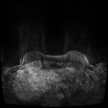
\includegraphics[width=4.2cm]{fig/samples/mri/mri_original.png} 
            & 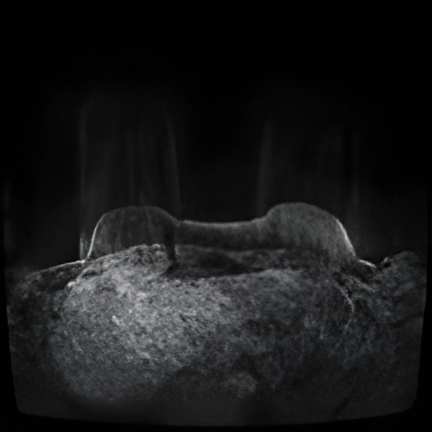
\includegraphics[width=4.2cm]{fig/samples/mri/mri_non_specific_training.png} 
            & 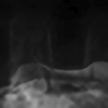
\includegraphics[width=4.2cm]{fig/samples/mri/mri_specific_training.png} \\
        (a) & (b) & (c)
    \end{tabular}
    \legend{Fonte: Autor}
    \label{fig:img-results:fig1}
\end{figure}


\begin{figure}[H]
    \centering
    \caption{Amostra aleatoriamente capturada das imagens de astronomia.}
    \begin{tabular}{c c c}
        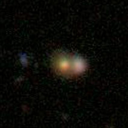
\includegraphics[width=4.2cm]{fig/samples/astronomy/astronomy_original.png} 
            & 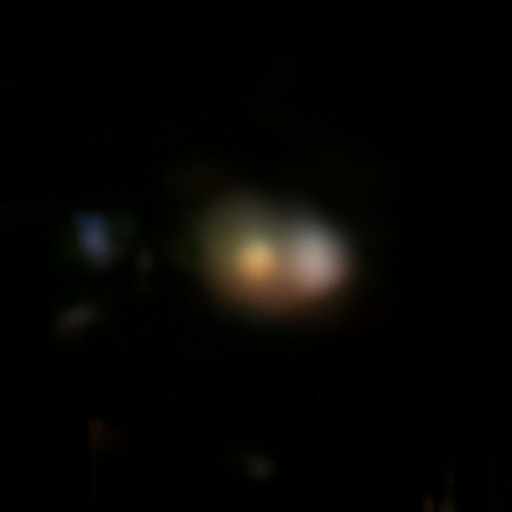
\includegraphics[width=4.2cm]{fig/samples/astronomy/astronomy_non_specific_training.png} 
            & 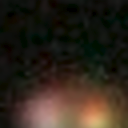
\includegraphics[width=4.2cm]{fig/samples/astronomy/astronomy_specific_training.png} \\
        (a) & (b) & (c)
    \end{tabular}
    \legend{Fonte: Autor}
    \label{fig:img-results:fig2}
\end{figure}

\section{Visualização dos resultados}
\label{sec:visualizacao-resultado}

Todas as imagens abaixo, possuem um gráfico superior, com os valores reais dos erros calculados, assim como uma regressão polinomial de primeiro grau e uma regressão polinomial de maior grau. Este gráfico está representado em escala logarítmica para os erros MSE e RMSE, devido à grande dispersão observada na visualização. Dessa forma, a imagem é mais compacta e concisa. 


A regressão de primeiro grau permite visualizar uma tendência geral dos dados e a regressão de maior grau aproximará ainda mais dos pontos distribuídos. As regressões fornecem uma melhor ideia de qual dos casos obteve um erro maior.

As imagens também possuem um histograma no gráfico inferior, representando a distribuição dos erros para ambos os cenários estudados, treinamento genérico e treinamento específico.

\subsection{Considerações gerais sobre os gráficos de resultados}
\label{sec:result:consideracoes-gerais}

Todas as imagens abaixo contém, no gráfico geral, os seguintes componentes:

\begin{itemize}
    \item Os pontos em azul, representando o valor do ETE.
    \item Os pontos em laranja, representando o valor do ETG.
    \item A estrela em vermelho, representando o valor mínimo do ETE.
    \item A estrela em azul, representando o valor mínimo do ETG.
    \item A estrela em amarelo, representando o valor máximo do ETE.
    \item A estrela em verde, representando o valor máximo do ETG.
    \item A curva em verde, representando o polinômio de primeiro grau, originado da regressão dos valores do ETE.
    \item A curva em vermelho escuro, representando o polinômio de primeiro grau, originado da regressão dos valores do ETG.
    \item A curva pontilhada em roxo, representando o polinômio de 40º grau, originado da regressão dos valores do ETE.
    \item A curva pontilhada em marrom, representando o polinômio de 40º grau, originado da regressão dos valores do ETG.
    \item Um histograma com a distribuição dos erros na parte inferior das imagens
\end{itemize}

\subsection{Estudo de resultados envolvendo a base de dados de ressonância magnética}
\label{sec:result:mri}
\subsubsection{Erro quadrático médio (MSE)}
\label{sec:result:mri:mse}

Começando com o erro quadrático médio, ao comparar a similaridade das imagens super resolvidas pela rede genericamente treinada com a similaridade das imagens super resolvidas pela rede treinada especificamente para lidar com imagens de ressonância magnética, são obtidos os resultados abaixo:

\begin{figure}[H]
    \centering
    \caption{Cálculo de erro MSE para base de dados de ressonância magnética.}
    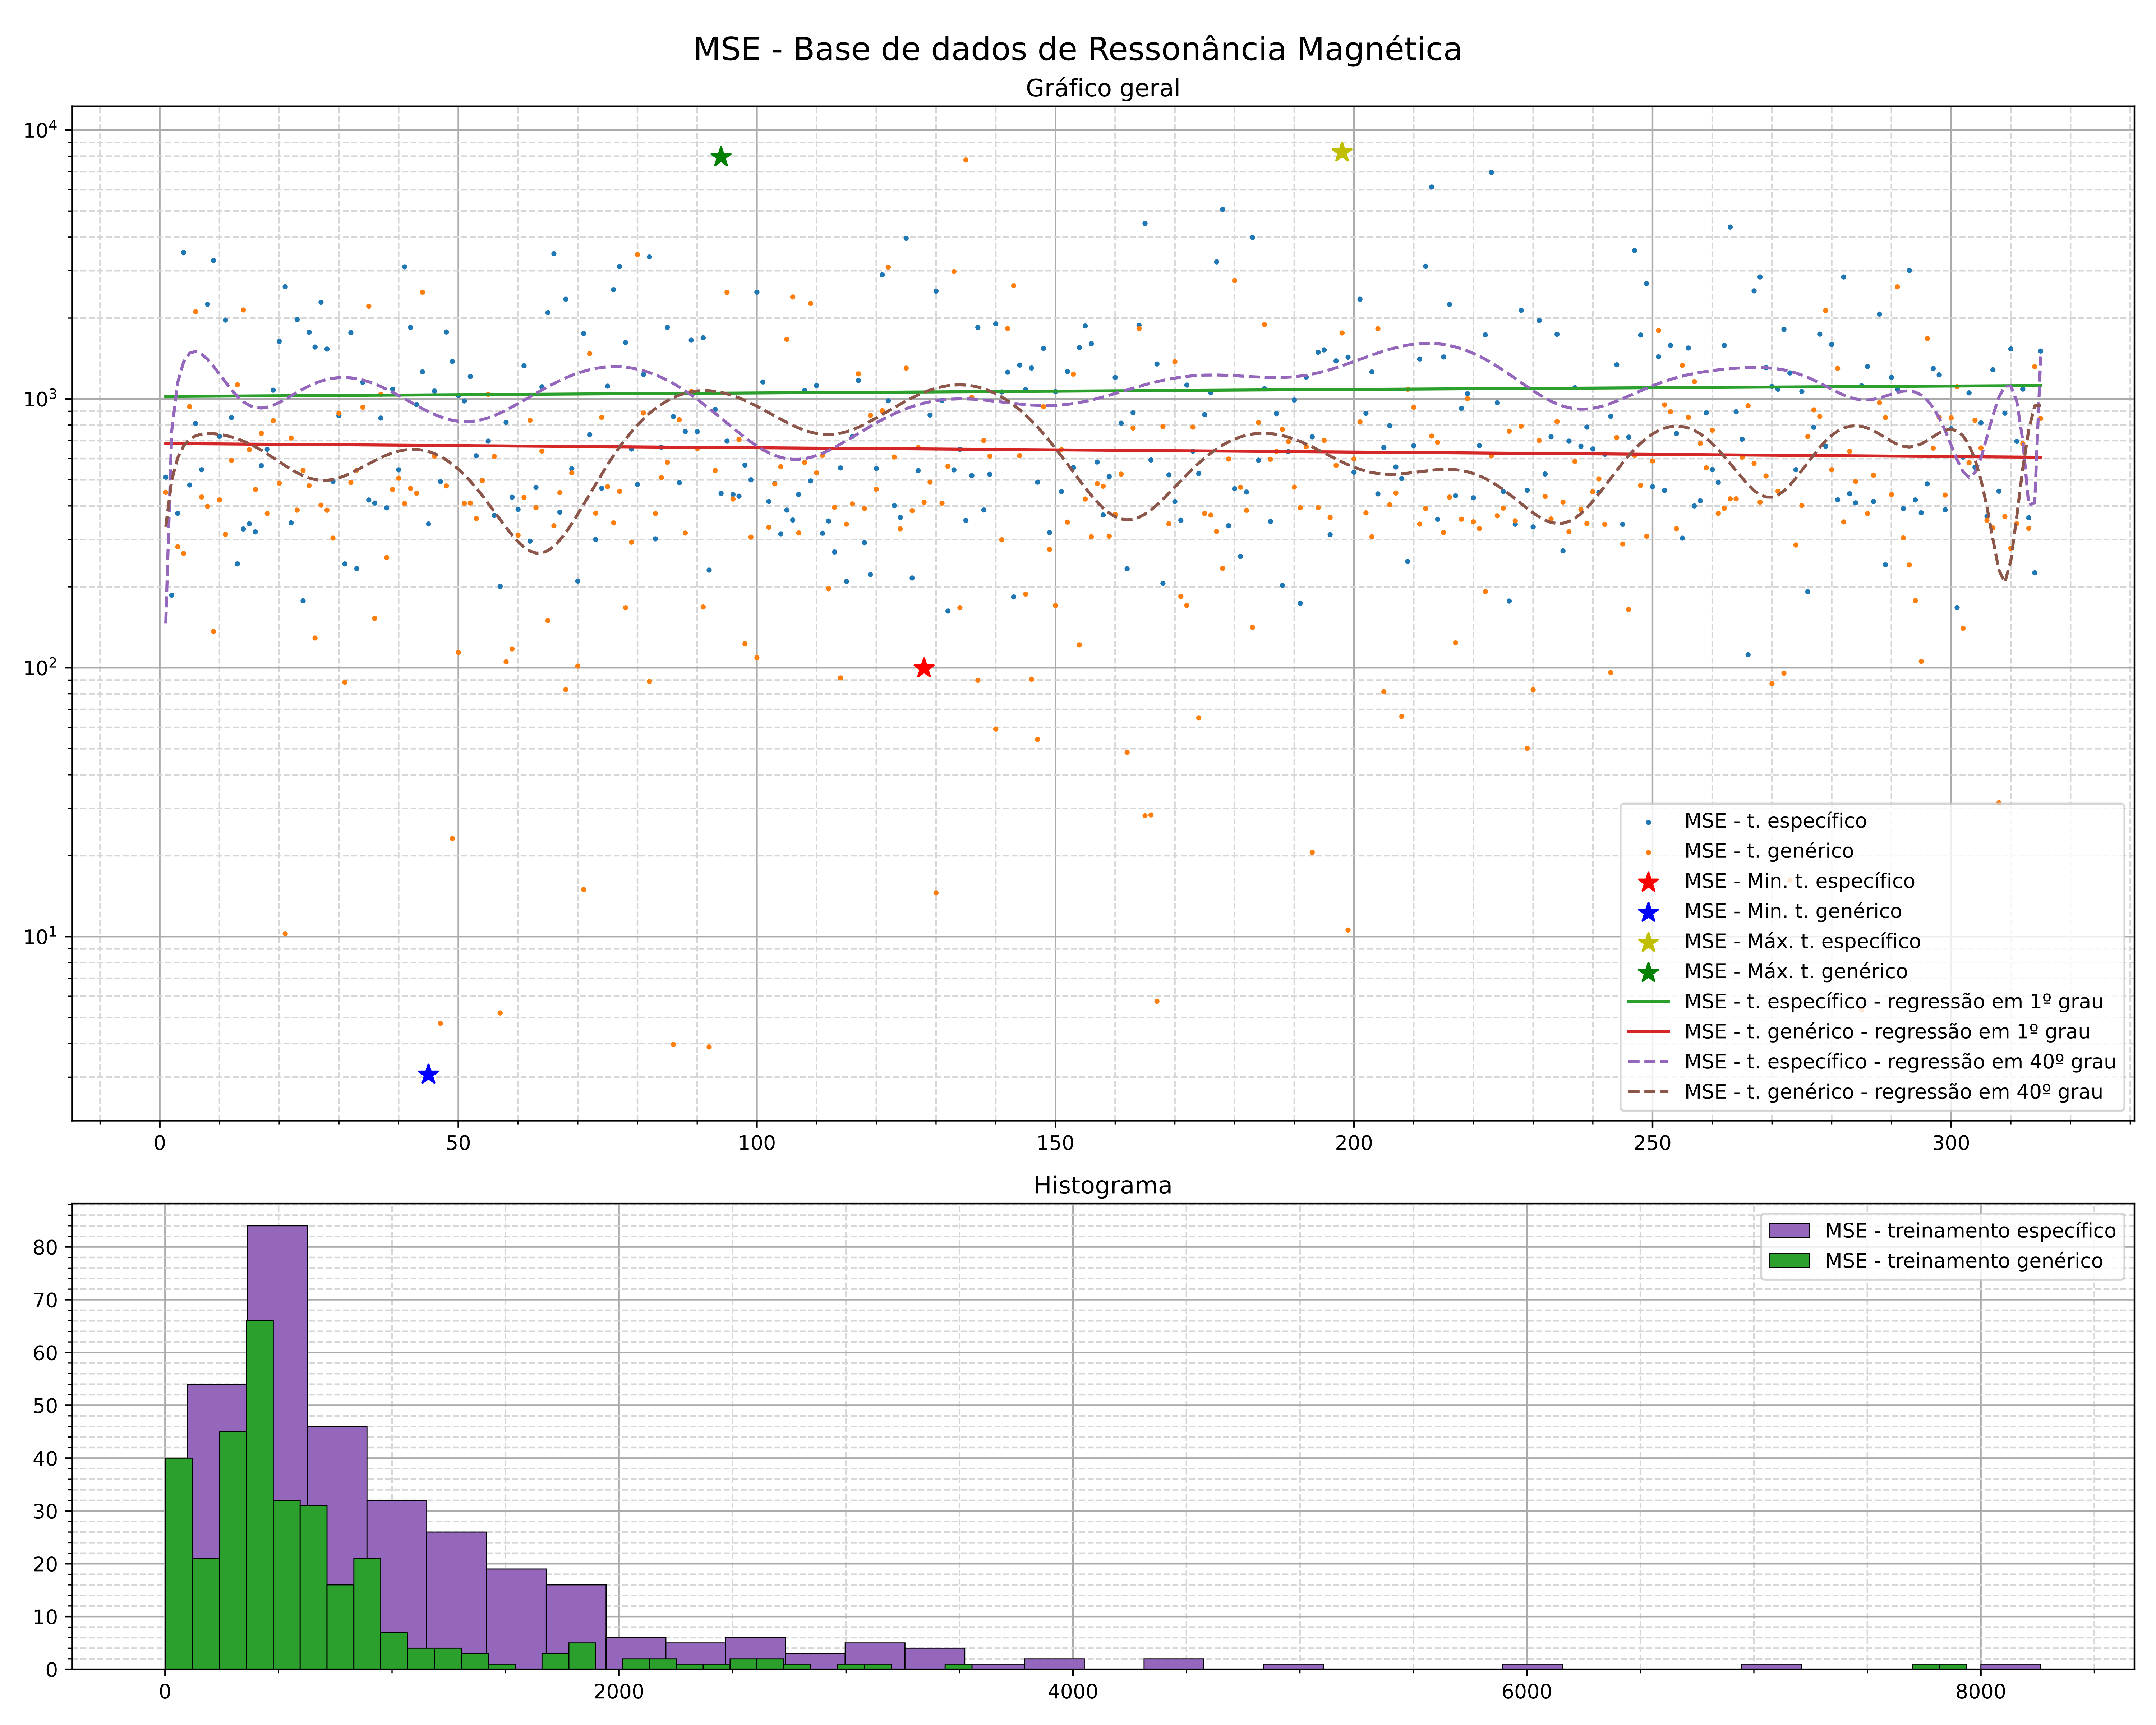
\includegraphics[width=10cm]{fig/resultados/mri/png/mse_mri_compound.png}
    \legend{Fonte: Autor}
    \label{fig:results:fig1}
\end{figure}

Os erros da figura \ref{fig:results:fig1} foram maiores nas imagens treinadas de forma específica. É notável que os polinômios relativos ao treinamento específico estão, em sua maior parte, acima dos polinômios do treinamento genérico. 

A mesma conclusão pode ser tirada, ao analisar a distribuição dos valores no histograma. A distribuição dos valores do ETE estão deslocadas mais à direita da distribuição do ETG. 


\subsubsection{Raiz do erro quadrático médio (RMSE)}
\label{sec:result:mri:rmse}


\begin{figure}[H]
    \centering
    \caption{Cálculo de erro RMSE para base de dados de ressonância magnética.}
    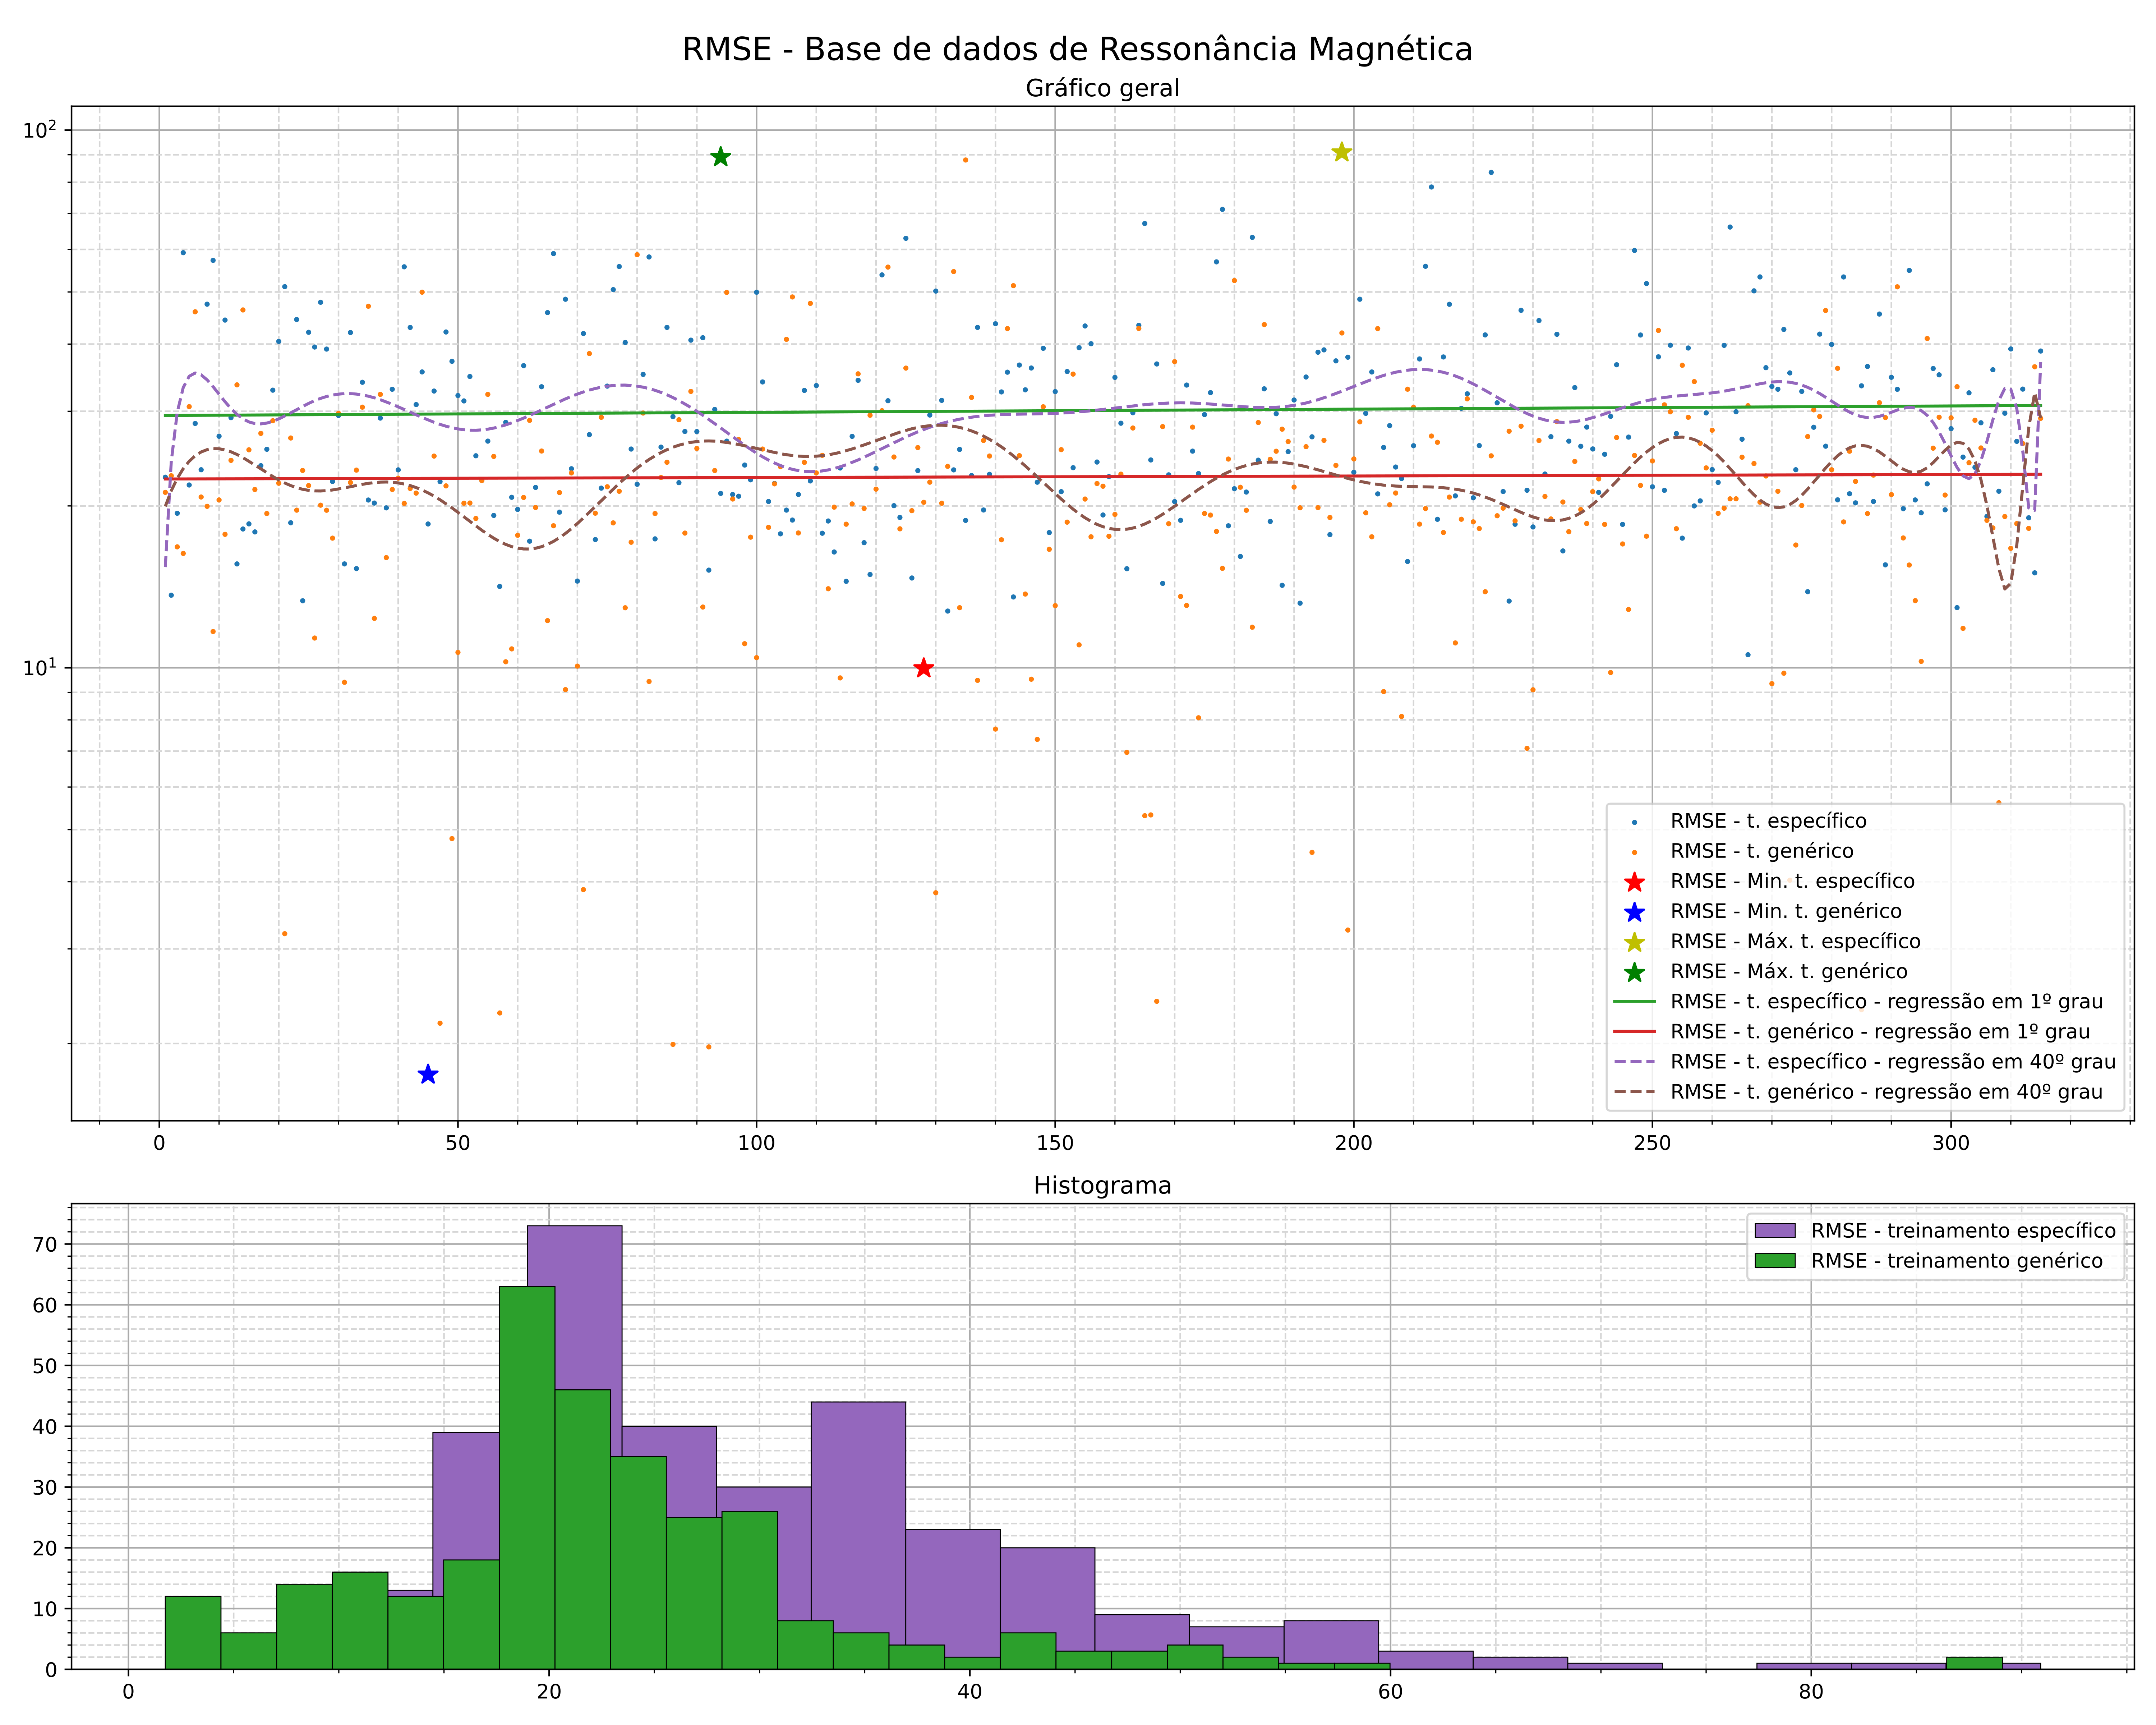
\includegraphics[width=10cm]{fig/resultados/mri/png/rmse_mri_compound.png}
    \legend{Fonte: Autor}
    \label{fig:results:fig2}
\end{figure}

O gráfico da figura \ref{fig:results:fig2} trás resultados muito similares aos da figura \ref{fig:results:fig1}, porém a variação do erro é menor. Enquanto no caso da figura \ref{fig:results:fig1} os valores se concentram entre 10 e 10000 para todas as amostras, para o erro RMSE, o intervalo é mais restrito: entre 0 e 100. Isso se deve à raiz quadrada, inexistente no cálculo do erro MSE.

Os resultados que podem ser extraídos do gráfico e histograma são praticamente idênticos aos extraídos da figura \ref{fig:results:fig1}. O treinamento específico da rede, produziu imagens com erros maiores que o treinamento genérico. 

\subsubsection{Relação sinal-ruído de pico (PSNR)}
\label{sec:result:mri:psnr}

\begin{figure}[H]
    \centering
    \caption{Cálculo de erro PSNR para base de dados de ressonância magnética.}
    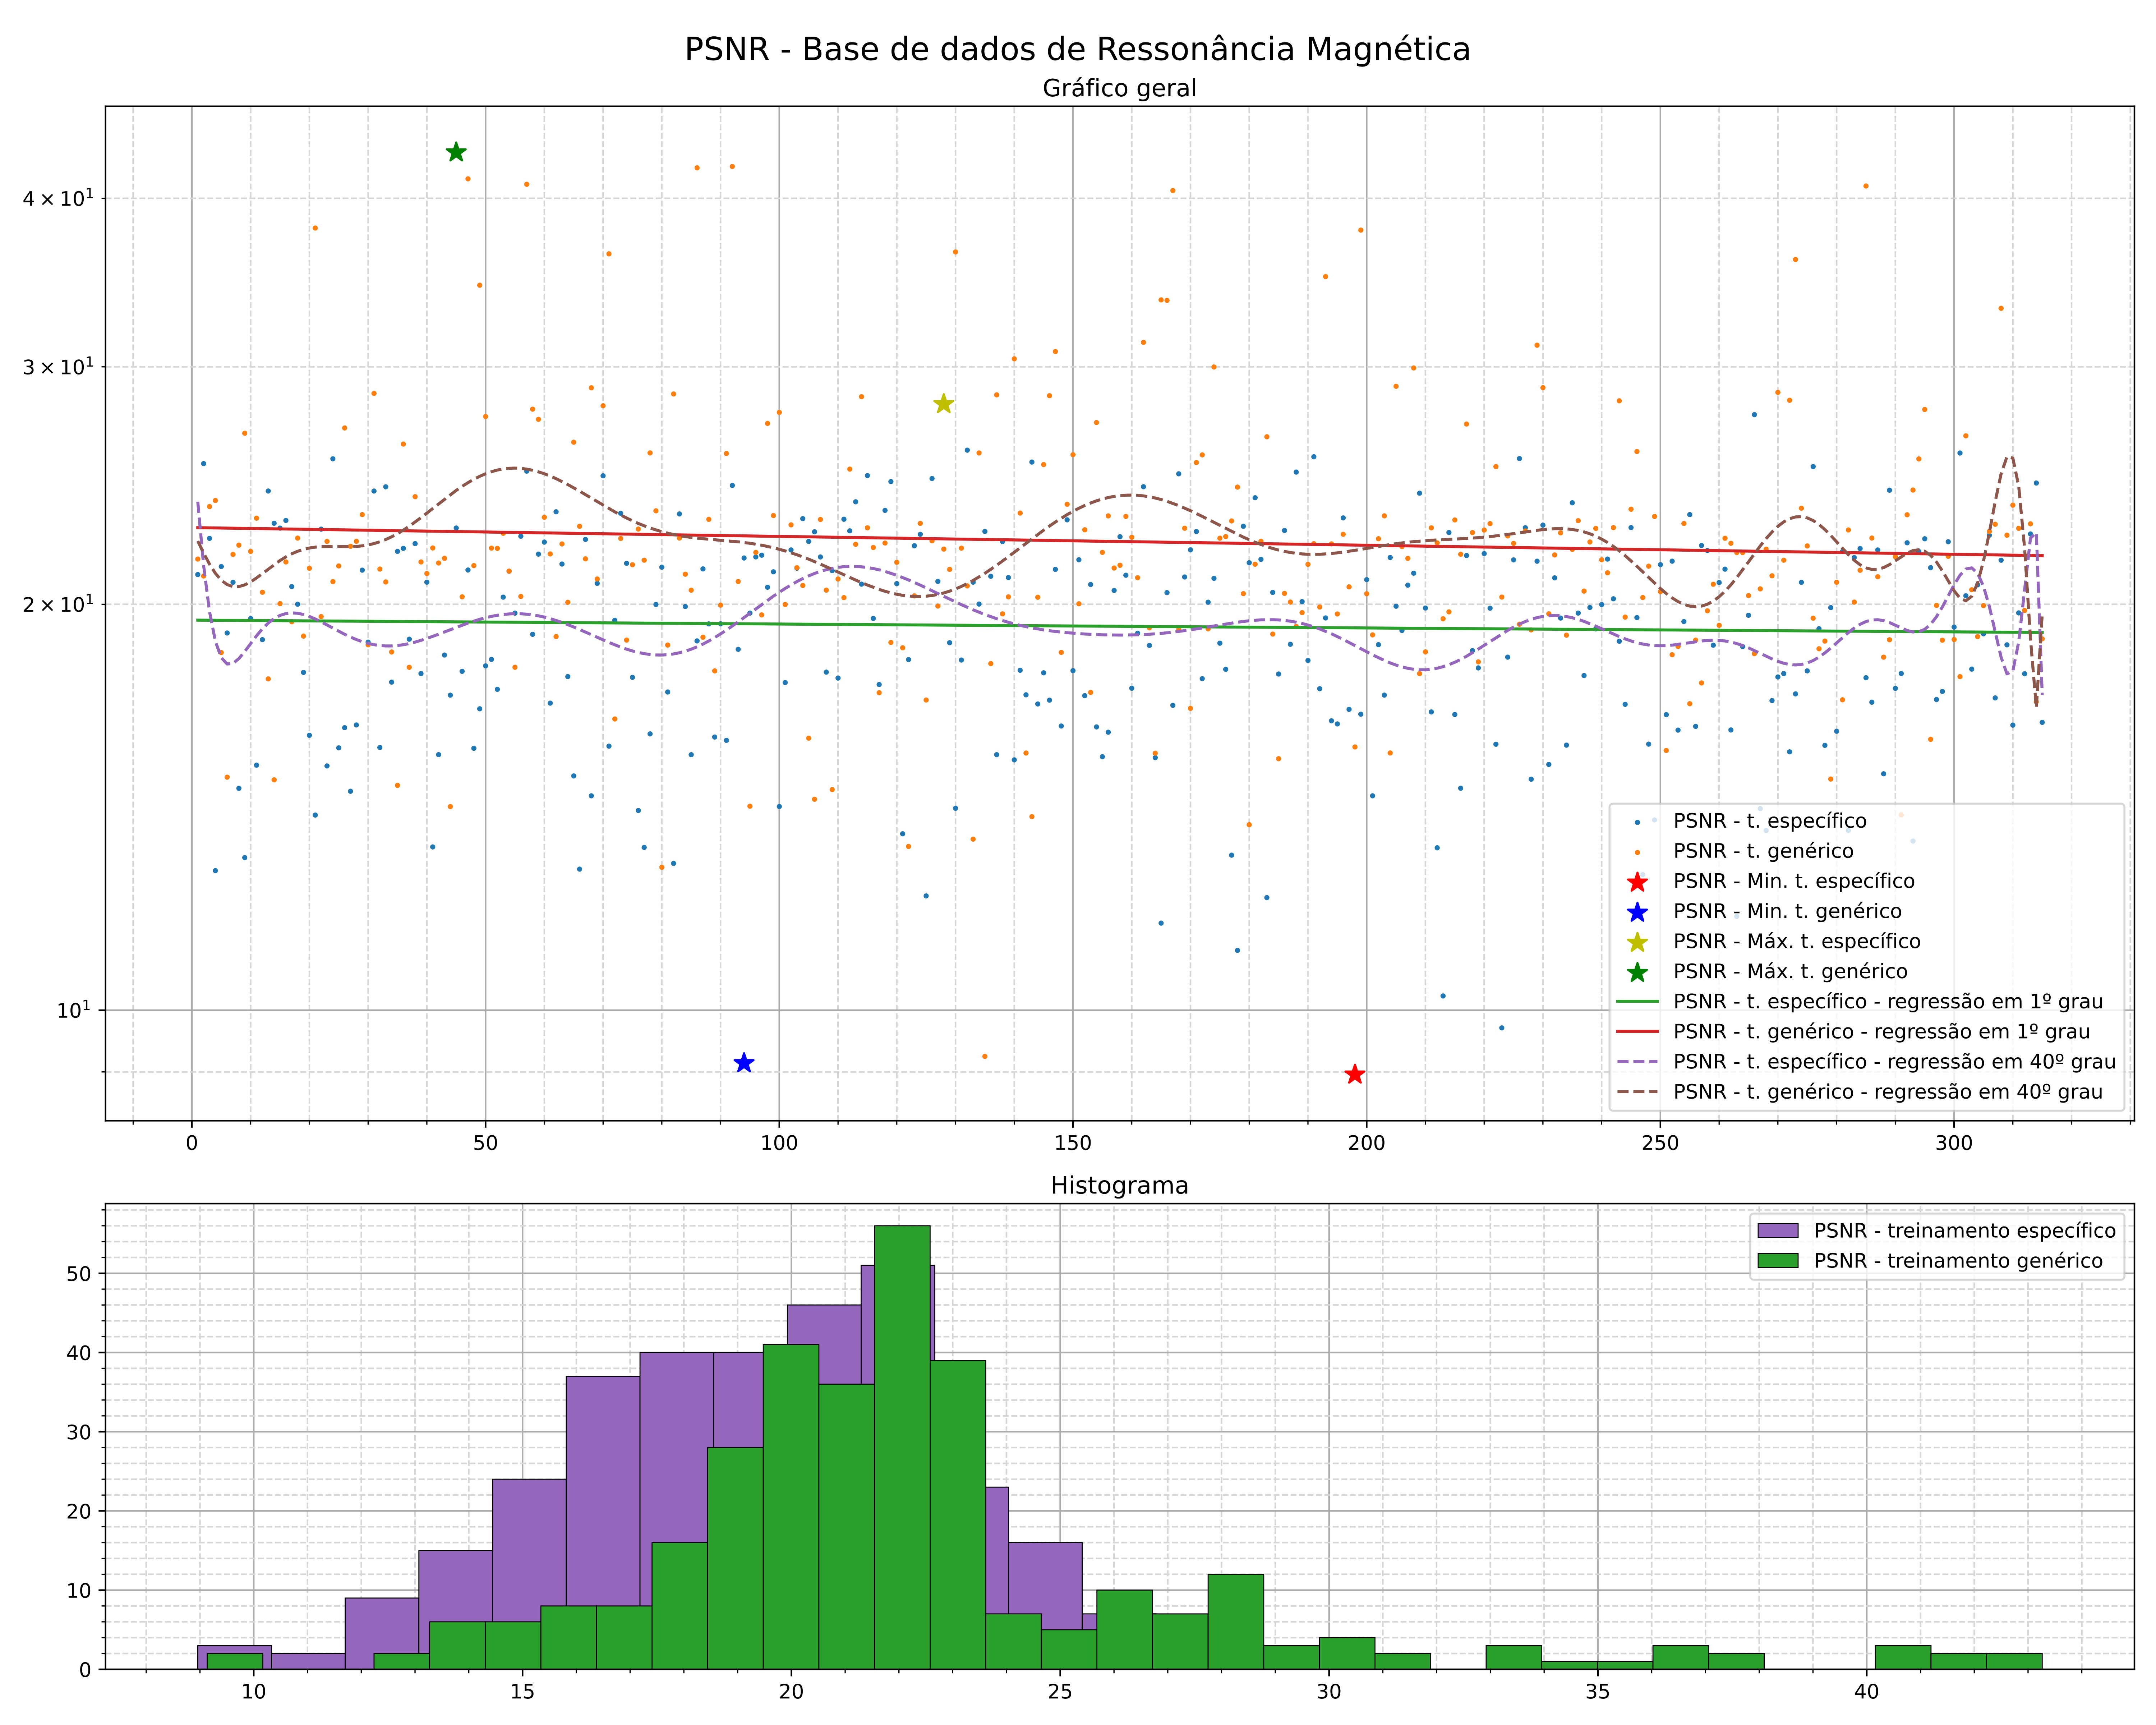
\includegraphics[width=10cm]{fig/resultados/mri/png/psnr_mri_compound.png}
    \legend{Fonte: Autor}
    \label{fig:results:fig3}
\end{figure}

Para esse erro em específico, a análise se inverte. Como descrito na seção \ref{sec:qualidade-imagem}, a similaridade entre as imagens é diretamente proporcional ao erro PSNR, enquanto nos casos anteriores a proporção era inversa.

Na figura \ref{fig:results:fig3}, mesmo utilizando uma escala logarítmica, observa-se bastante variação nas amostras. Seria difícil extrair significado destes dados sem as regressões polinomiais, dada tamanha dispersão. 

Com as regressões, nota-se que o treinamento específico produziu erros PSNR mais próximos de zero em relação ao treinamento genérico. O histograma confirma esta análise, demonstrando o deslocamento à esquerda das amostras do treinamento específico.

\subsubsection{Erro adimensional de síntese global relativa (ERGAS)}
\label{sec:result:mri:ergas}

\begin{figure}[H]
    \centering
    \caption{Cálculo de erro ERGAS para base de dados de ressonância magnética.}
    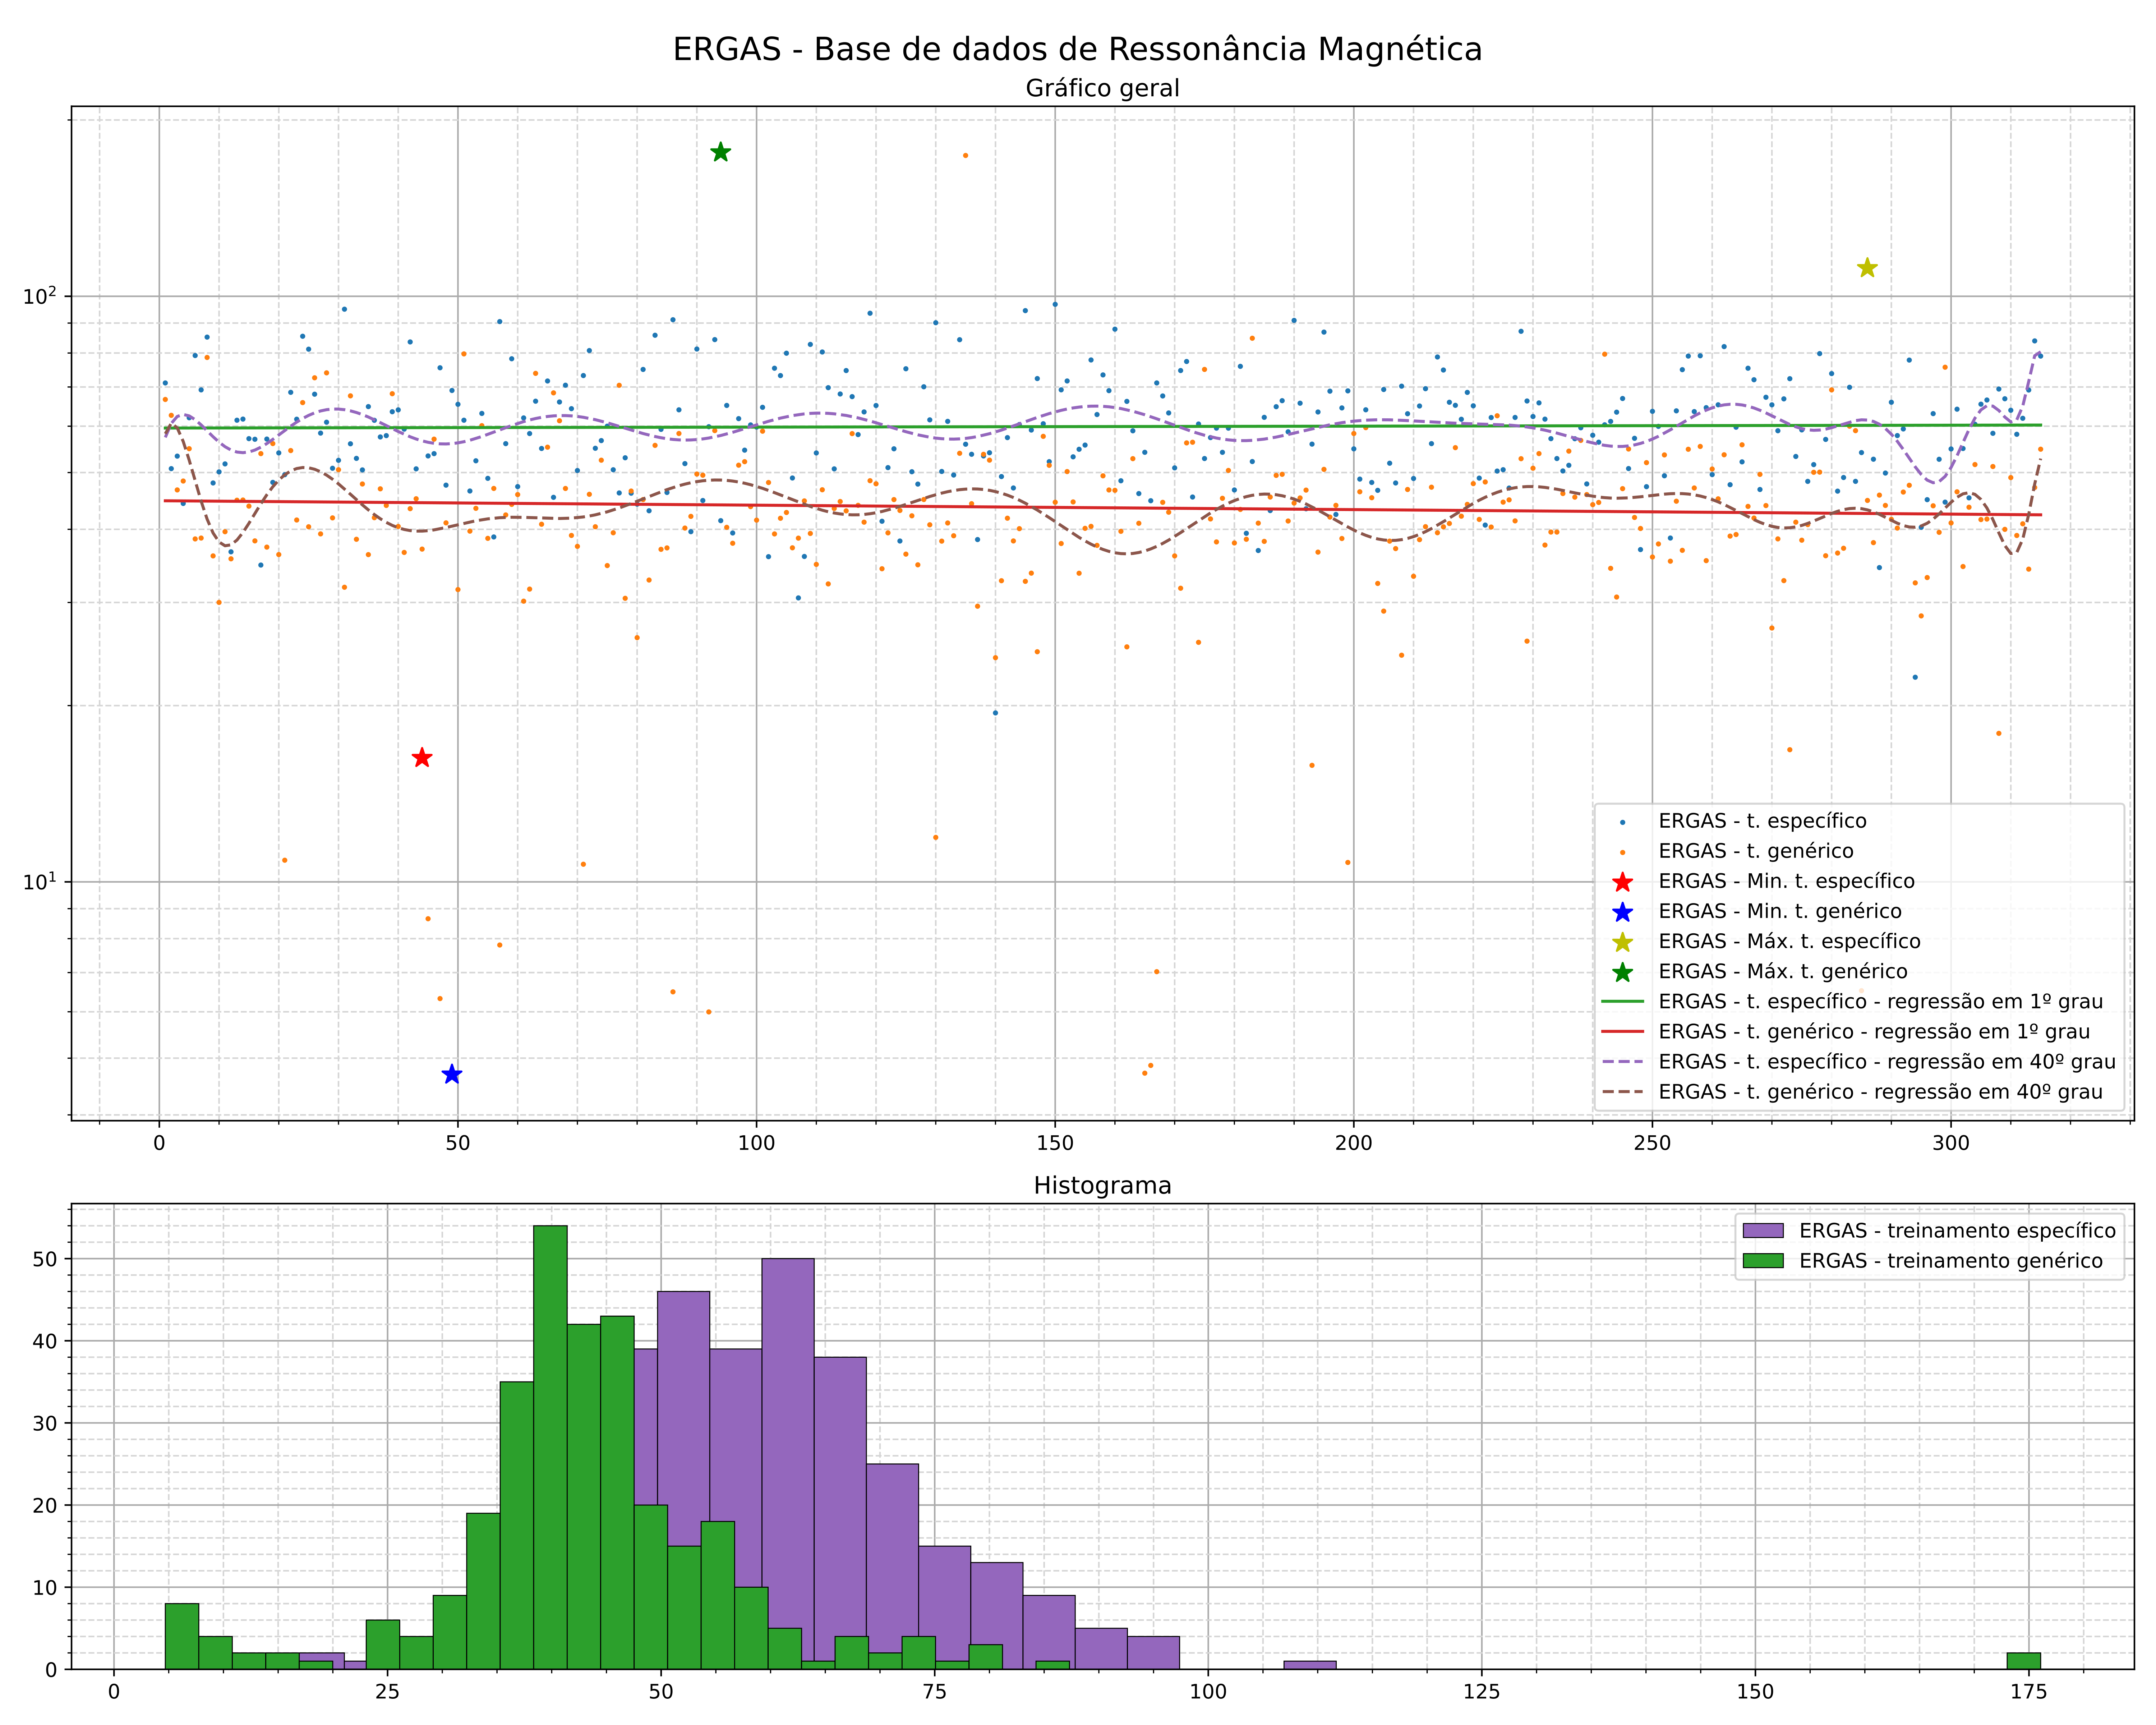
\includegraphics[width=10cm]{fig/resultados/mri/png/ergas_mri_compound.png}
    \legend{Fonte: Autor}
    \label{fig:results:fig4}
\end{figure}

O erro ERGAS da figura \ref{fig:results:fig4}, também produziu agrupamentos de amostras, mas dentro dos grupos, houve bastante variação entre os valores. Com as curvas de regressão no entanto, podemos claramente observar que o treinamento específico, novamente produziu erros maiores que o treinamento genérico. 

Assim como nas figuras \ref{fig:results:fig1} e \ref{fig:results:fig2}, a distribuição das amostras do ETE ficaram deslocadas à direita, evidenciando ainda mais o resultado antes descrito.

\subsection{Estudo de resultados envolvendo a base de dados de astronomia}
\label{sec:result:astronomy}

\subsubsection{Erro quadrático médio (MSE)}
\label{sec:result:astronomy:mse}

\begin{figure}[H]
    \centering
    \caption{Cálculo de erro MSE para base de dados astronômica.}
    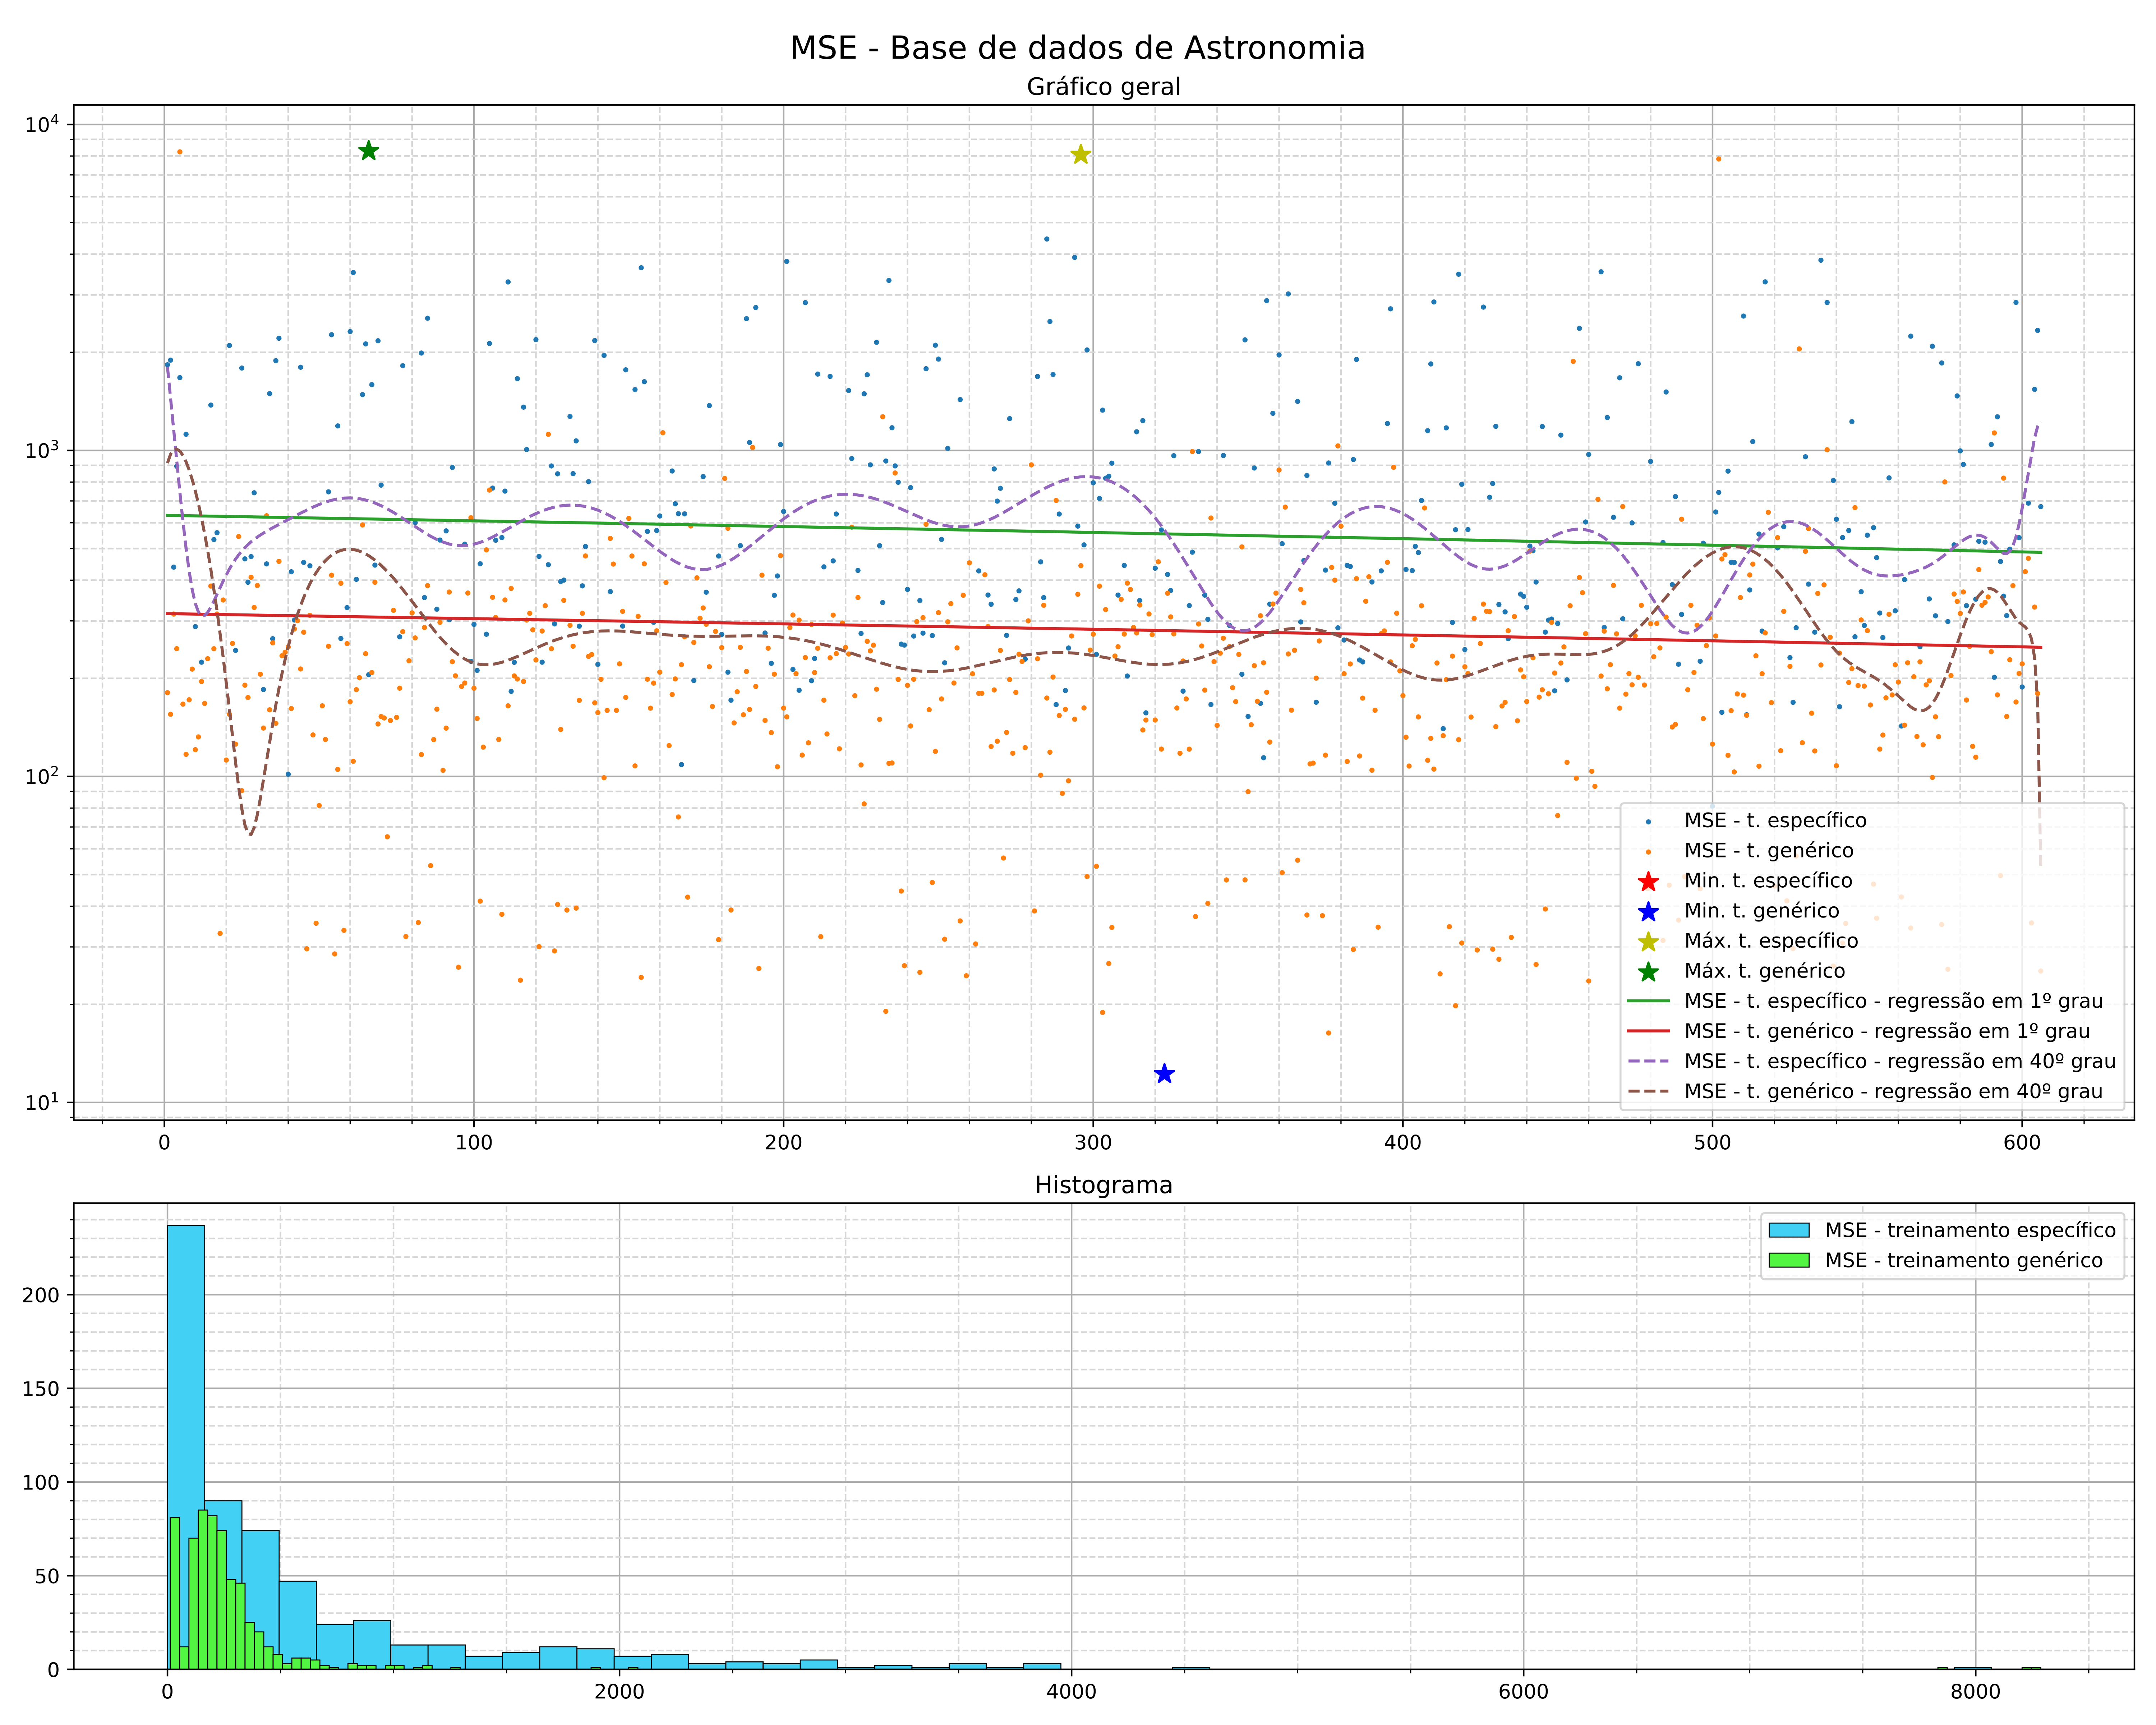
\includegraphics[width=10cm]{fig/resultados/astronomy/png/mse_astronomy_compound.png}
    \legend{Fonte: Autor}
    \label{fig:results:fig5}
\end{figure}

Na figura \ref{fig:results:fig5}, percebe-se com as regressões e o histograma que o ETE foi em sua maior parte, maior que o ETG. A distribuição do ETE se desloca à direita da distribuição do ETG.

\subsubsection{Raiz do erro quadrático médio (RMSE)}
\label{sec:result:astronomy:rmse}

\begin{figure}[H]
    \centering
    \caption{Cálculo de erro RMSE para base de dados astronômica.}
    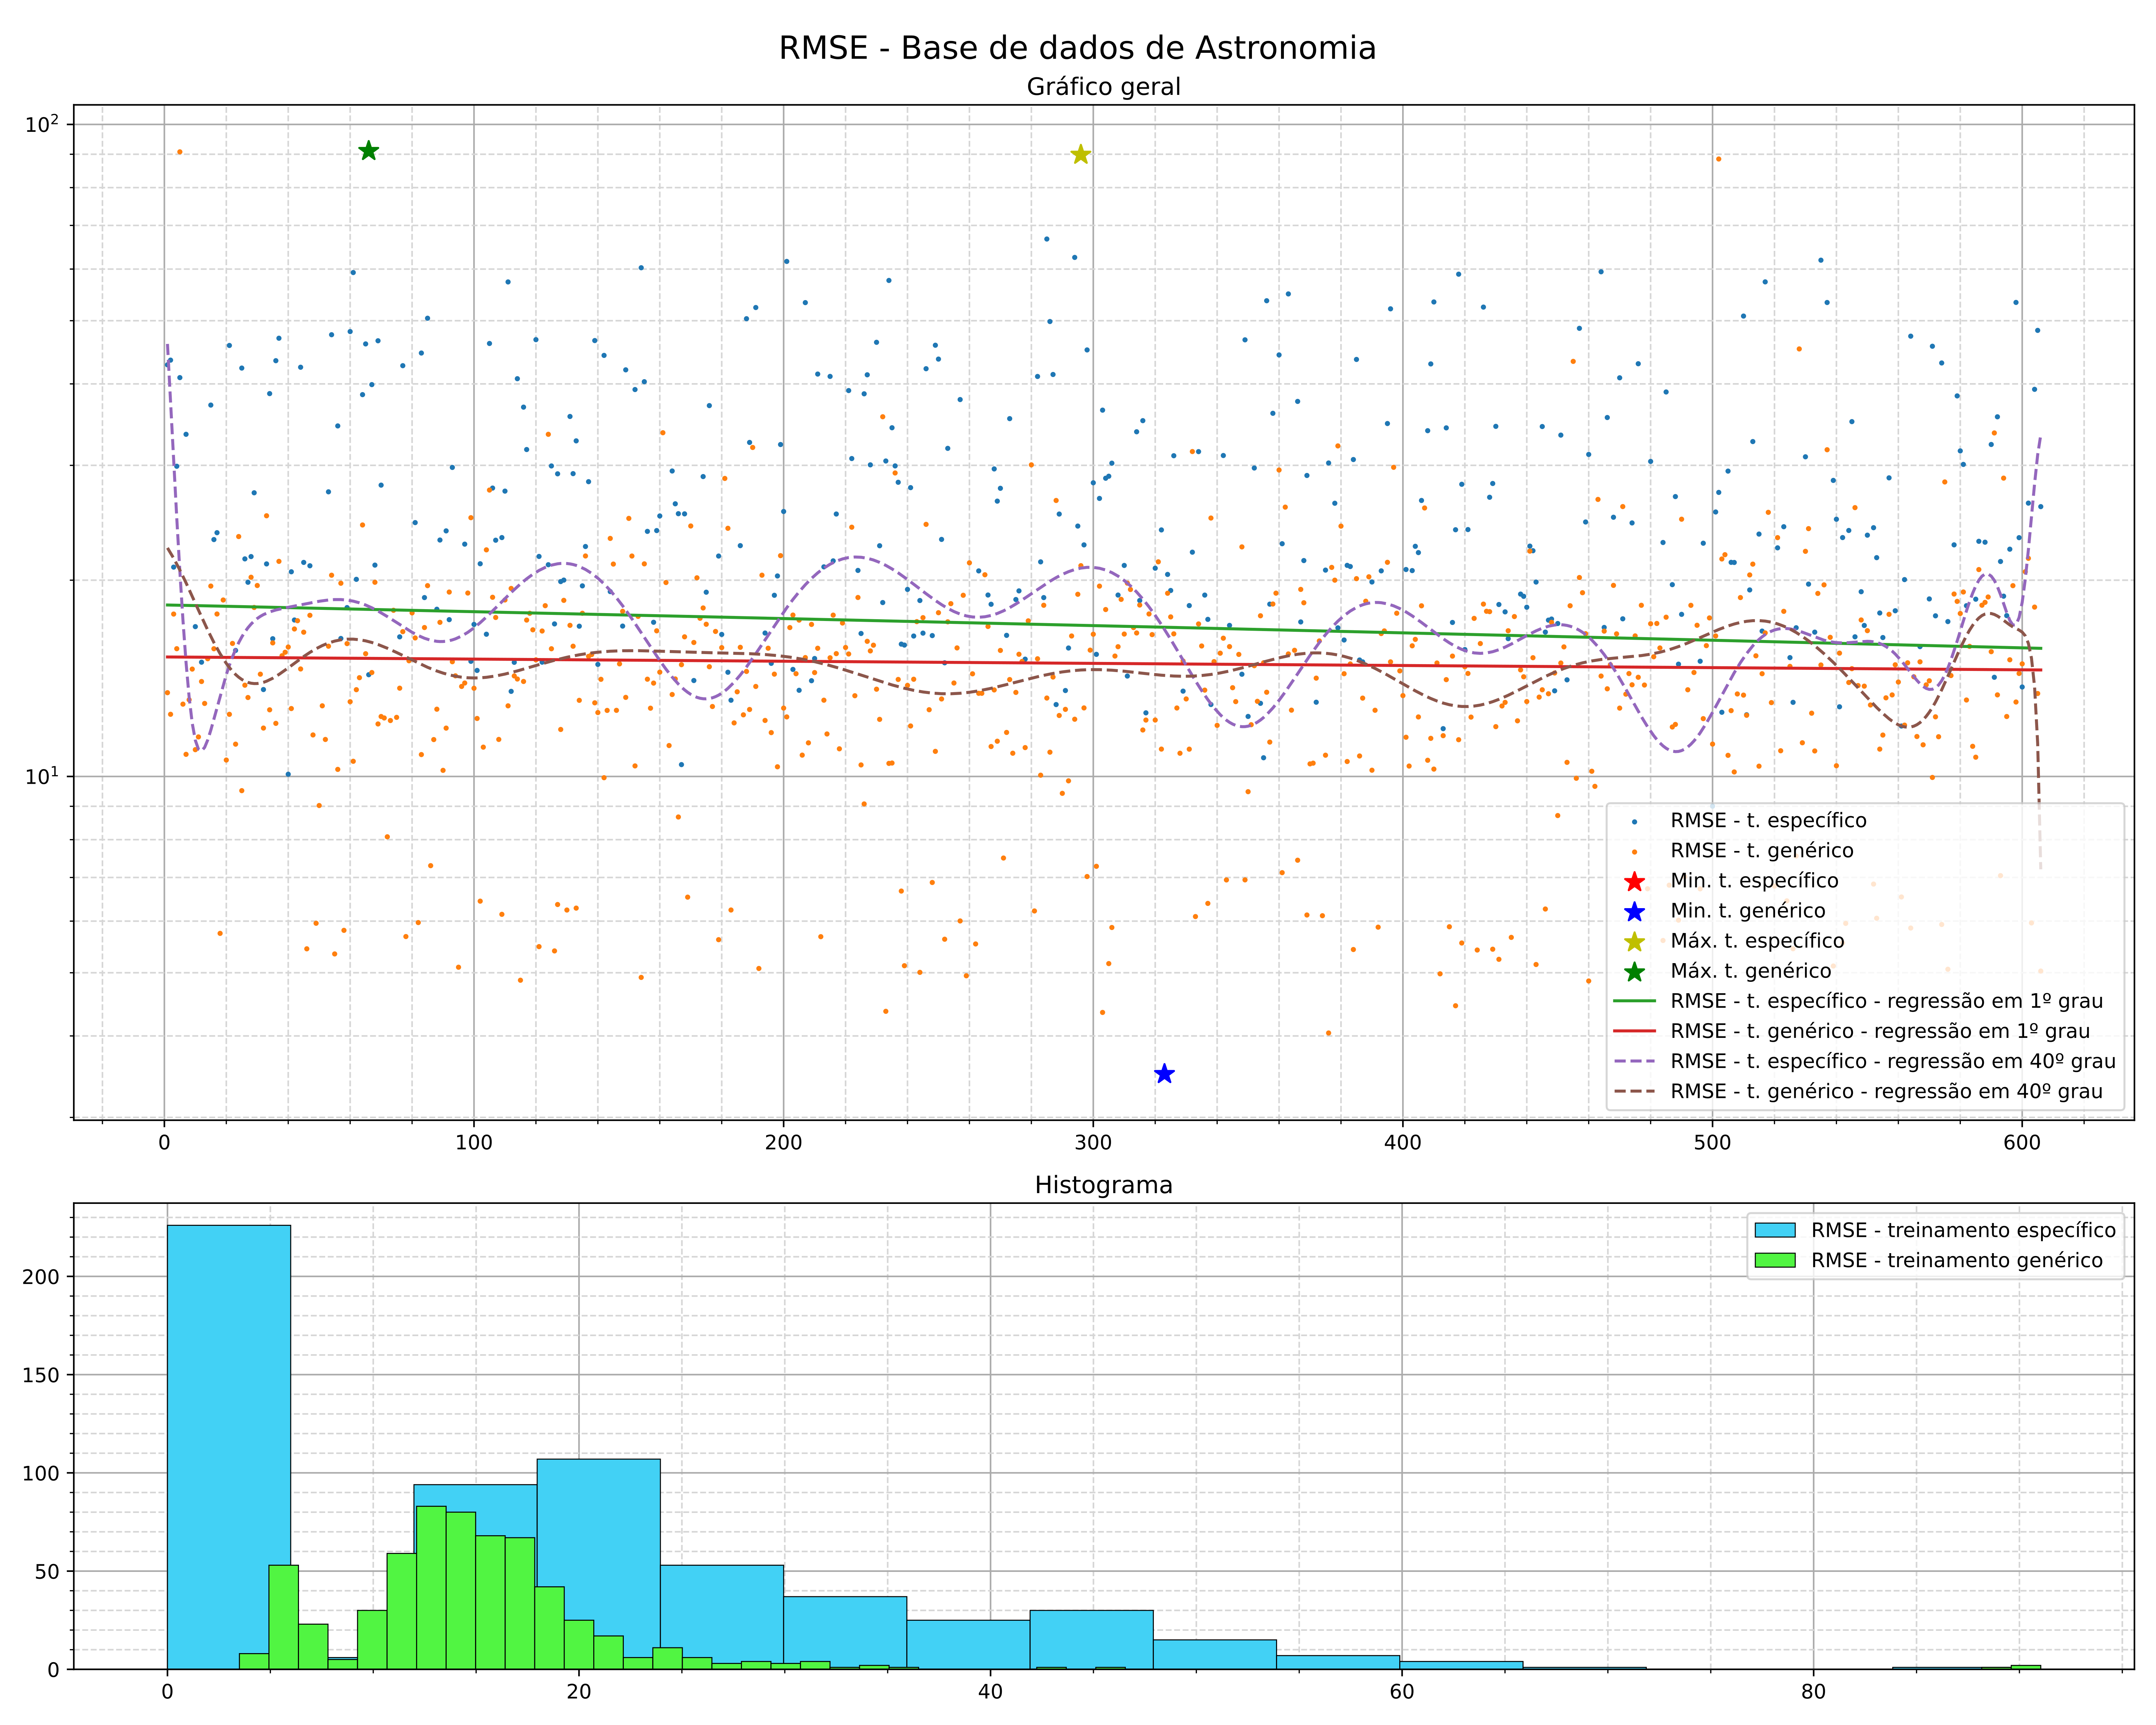
\includegraphics[width=10cm]{fig/resultados/astronomy/png/rmse_astronomy_compound.png}
    \legend{Fonte: Autor}
    \label{fig:results:fig6}
\end{figure}

A figura \ref{fig:results:fig6} traz resultados similares aos da figura \ref{fig:results:fig5}: o ETE é maior que o ETG. A principal diferença, como explicado anteriormente é o intervalo de distribuição reduzido de ambos os erros em relação à figura \ref{fig:results:fig5}.

\subsubsection{Relação sinal-ruído de pico (PSNR)}
\label{sec:result:astronomy:psnr}

\begin{figure}[H]
    \centering
    \caption{Cálculo de erro PSNR para base de dados astronômica.}
    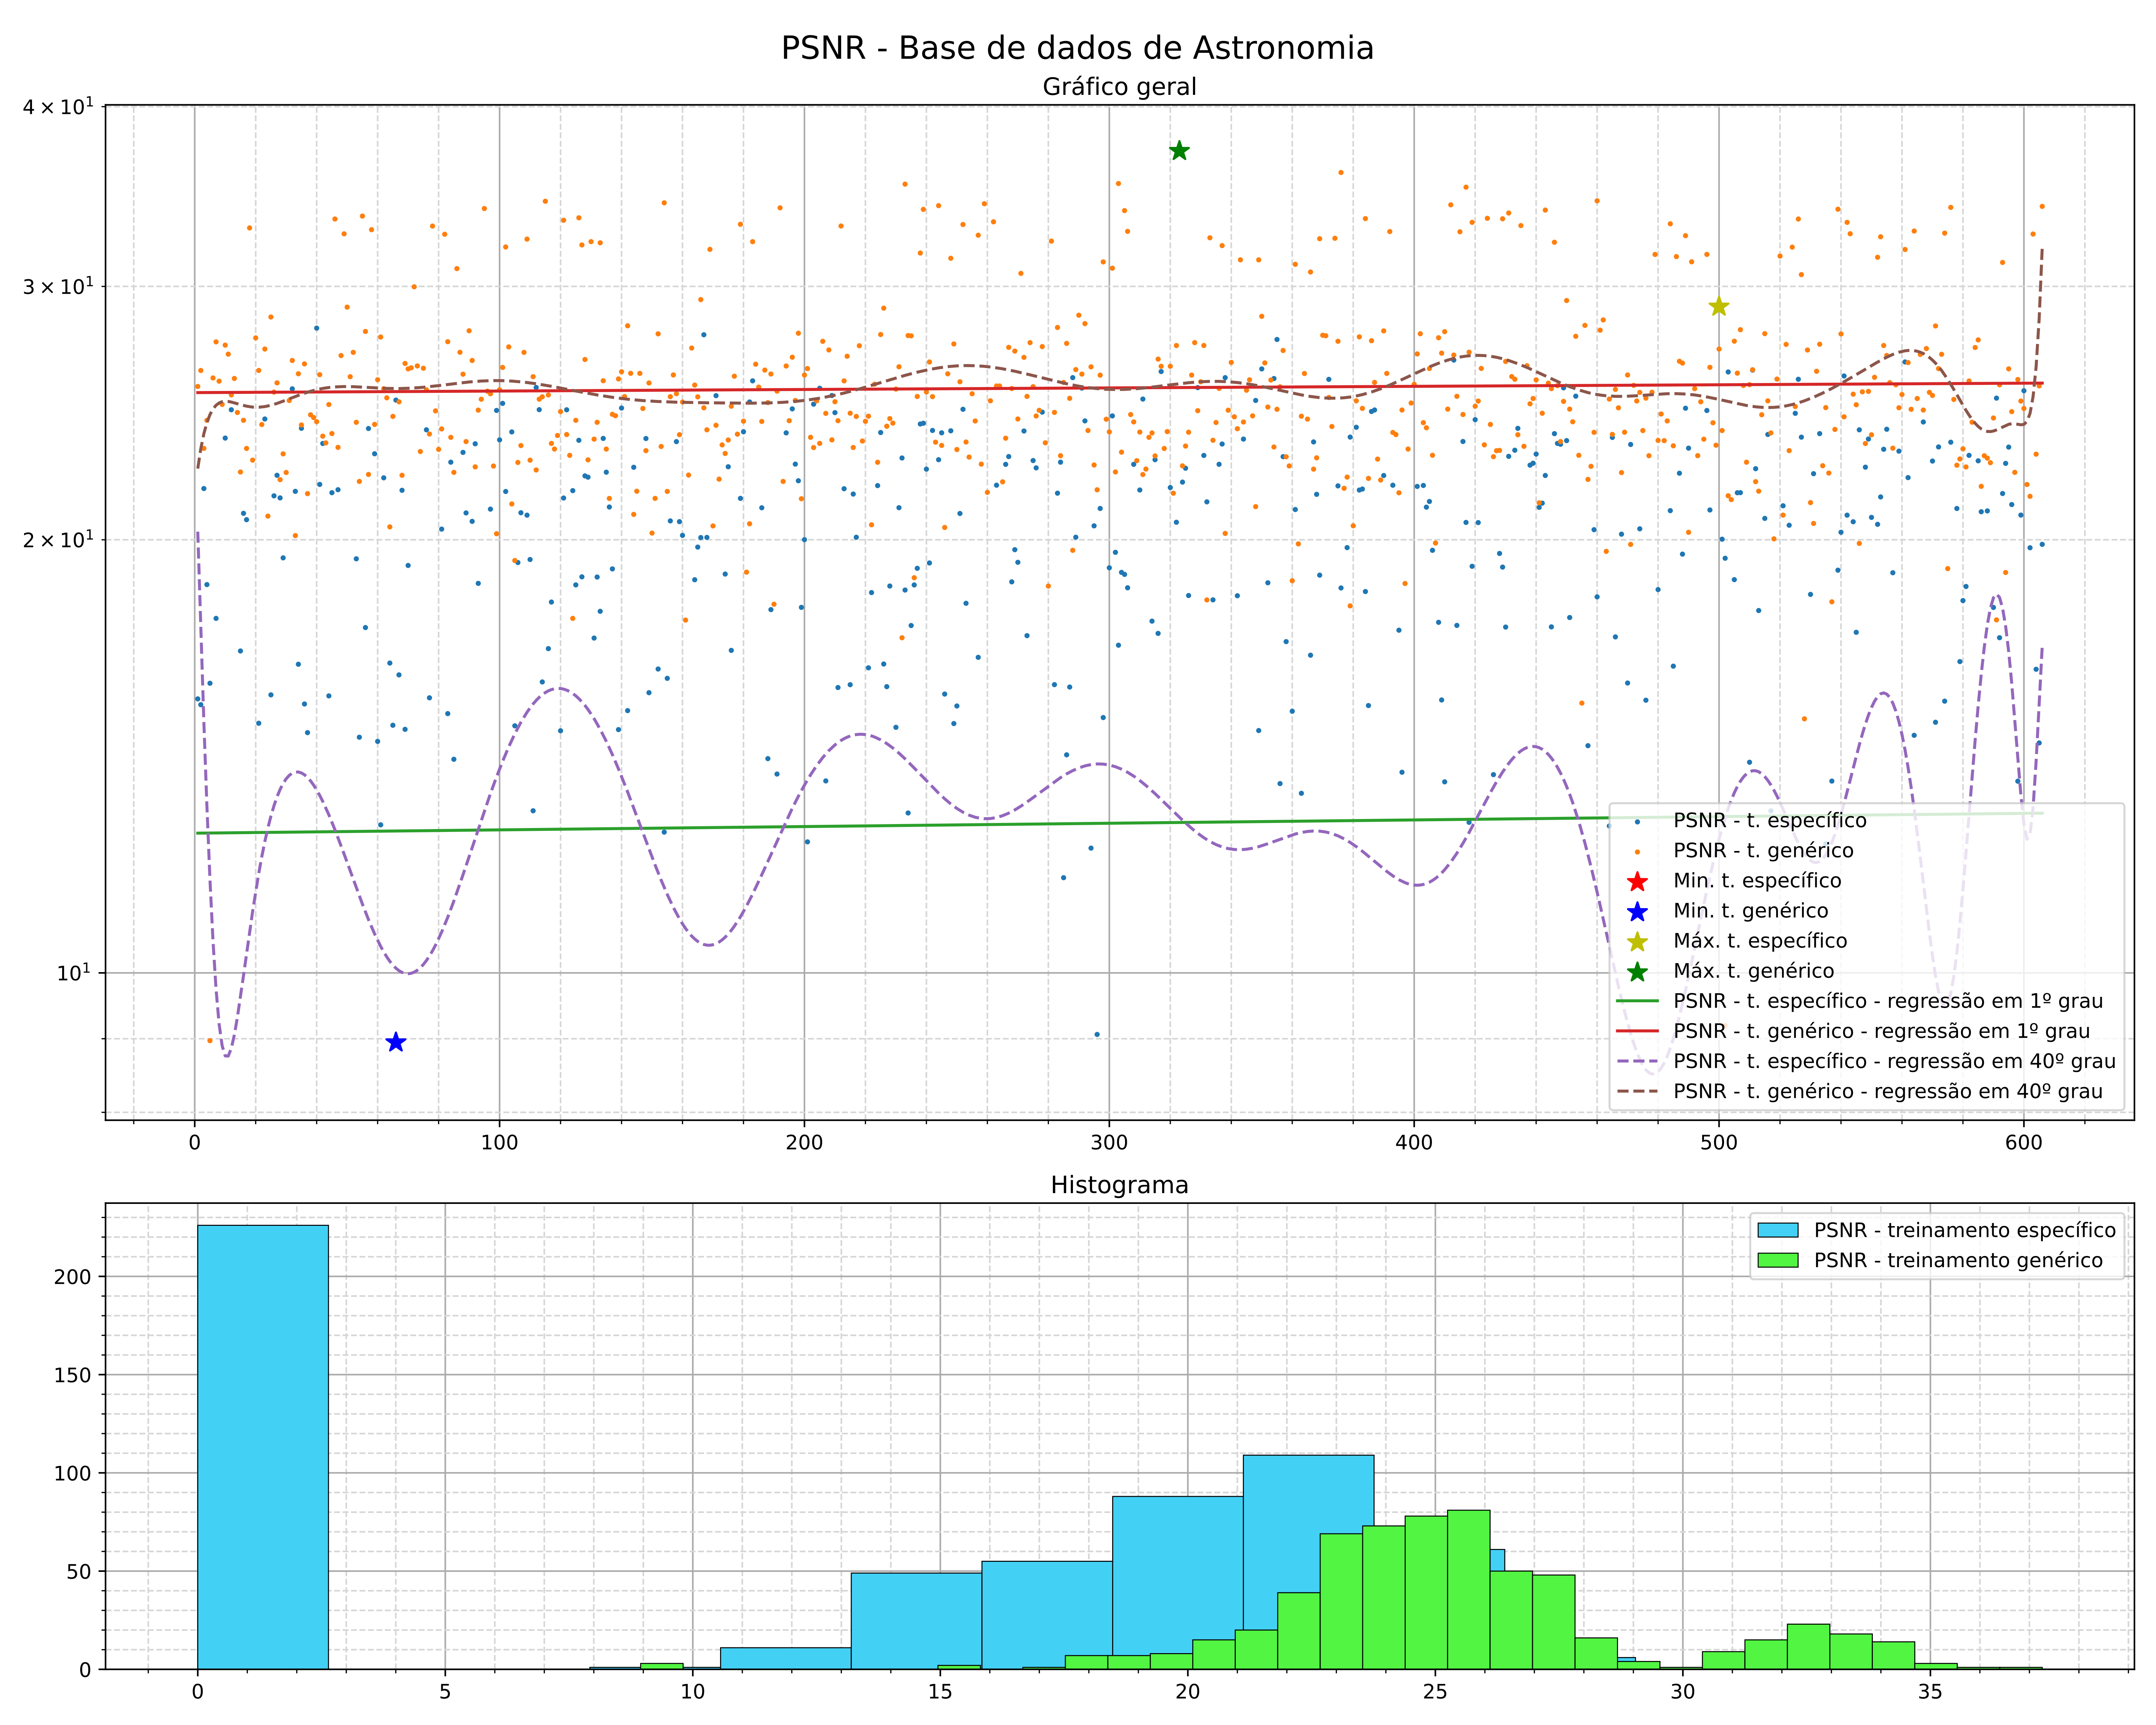
\includegraphics[width=10cm]{fig/resultados/astronomy/png/psnr_astronomy_compound.png}
    \legend{Fonte: Autor}
    \label{fig:results:fig7}
\end{figure}

No gráfico da figura \ref{fig:results:fig7} é possível observar que os dois cenários formam agrupamentos. O ETE está deslocado para baixo do gráfico. O resultado extraído disso são condizentes com o que foi visto nos erros anteriores. O treinamento específico gerou erros PSNR mais próximos de zero e estão distribuídos mais à esquerda dos erros do treinamento genérico.

Note também que o distanciamento entre as regressões do ETE e as regressões do ETG foi maior, em relação ao erro PSNR calculado para a base de dados de ressonância magnética na seção \ref{sec:result:mri:psnr}. 

\subsubsection{Erro adimensional de síntese global relativa (ERGAS)}
\label{sec:result:astronomy:ergas}

\begin{figure}[H]
    \centering
    \caption{Cálculo de erro ERGAS para base de dados astronômica.}
    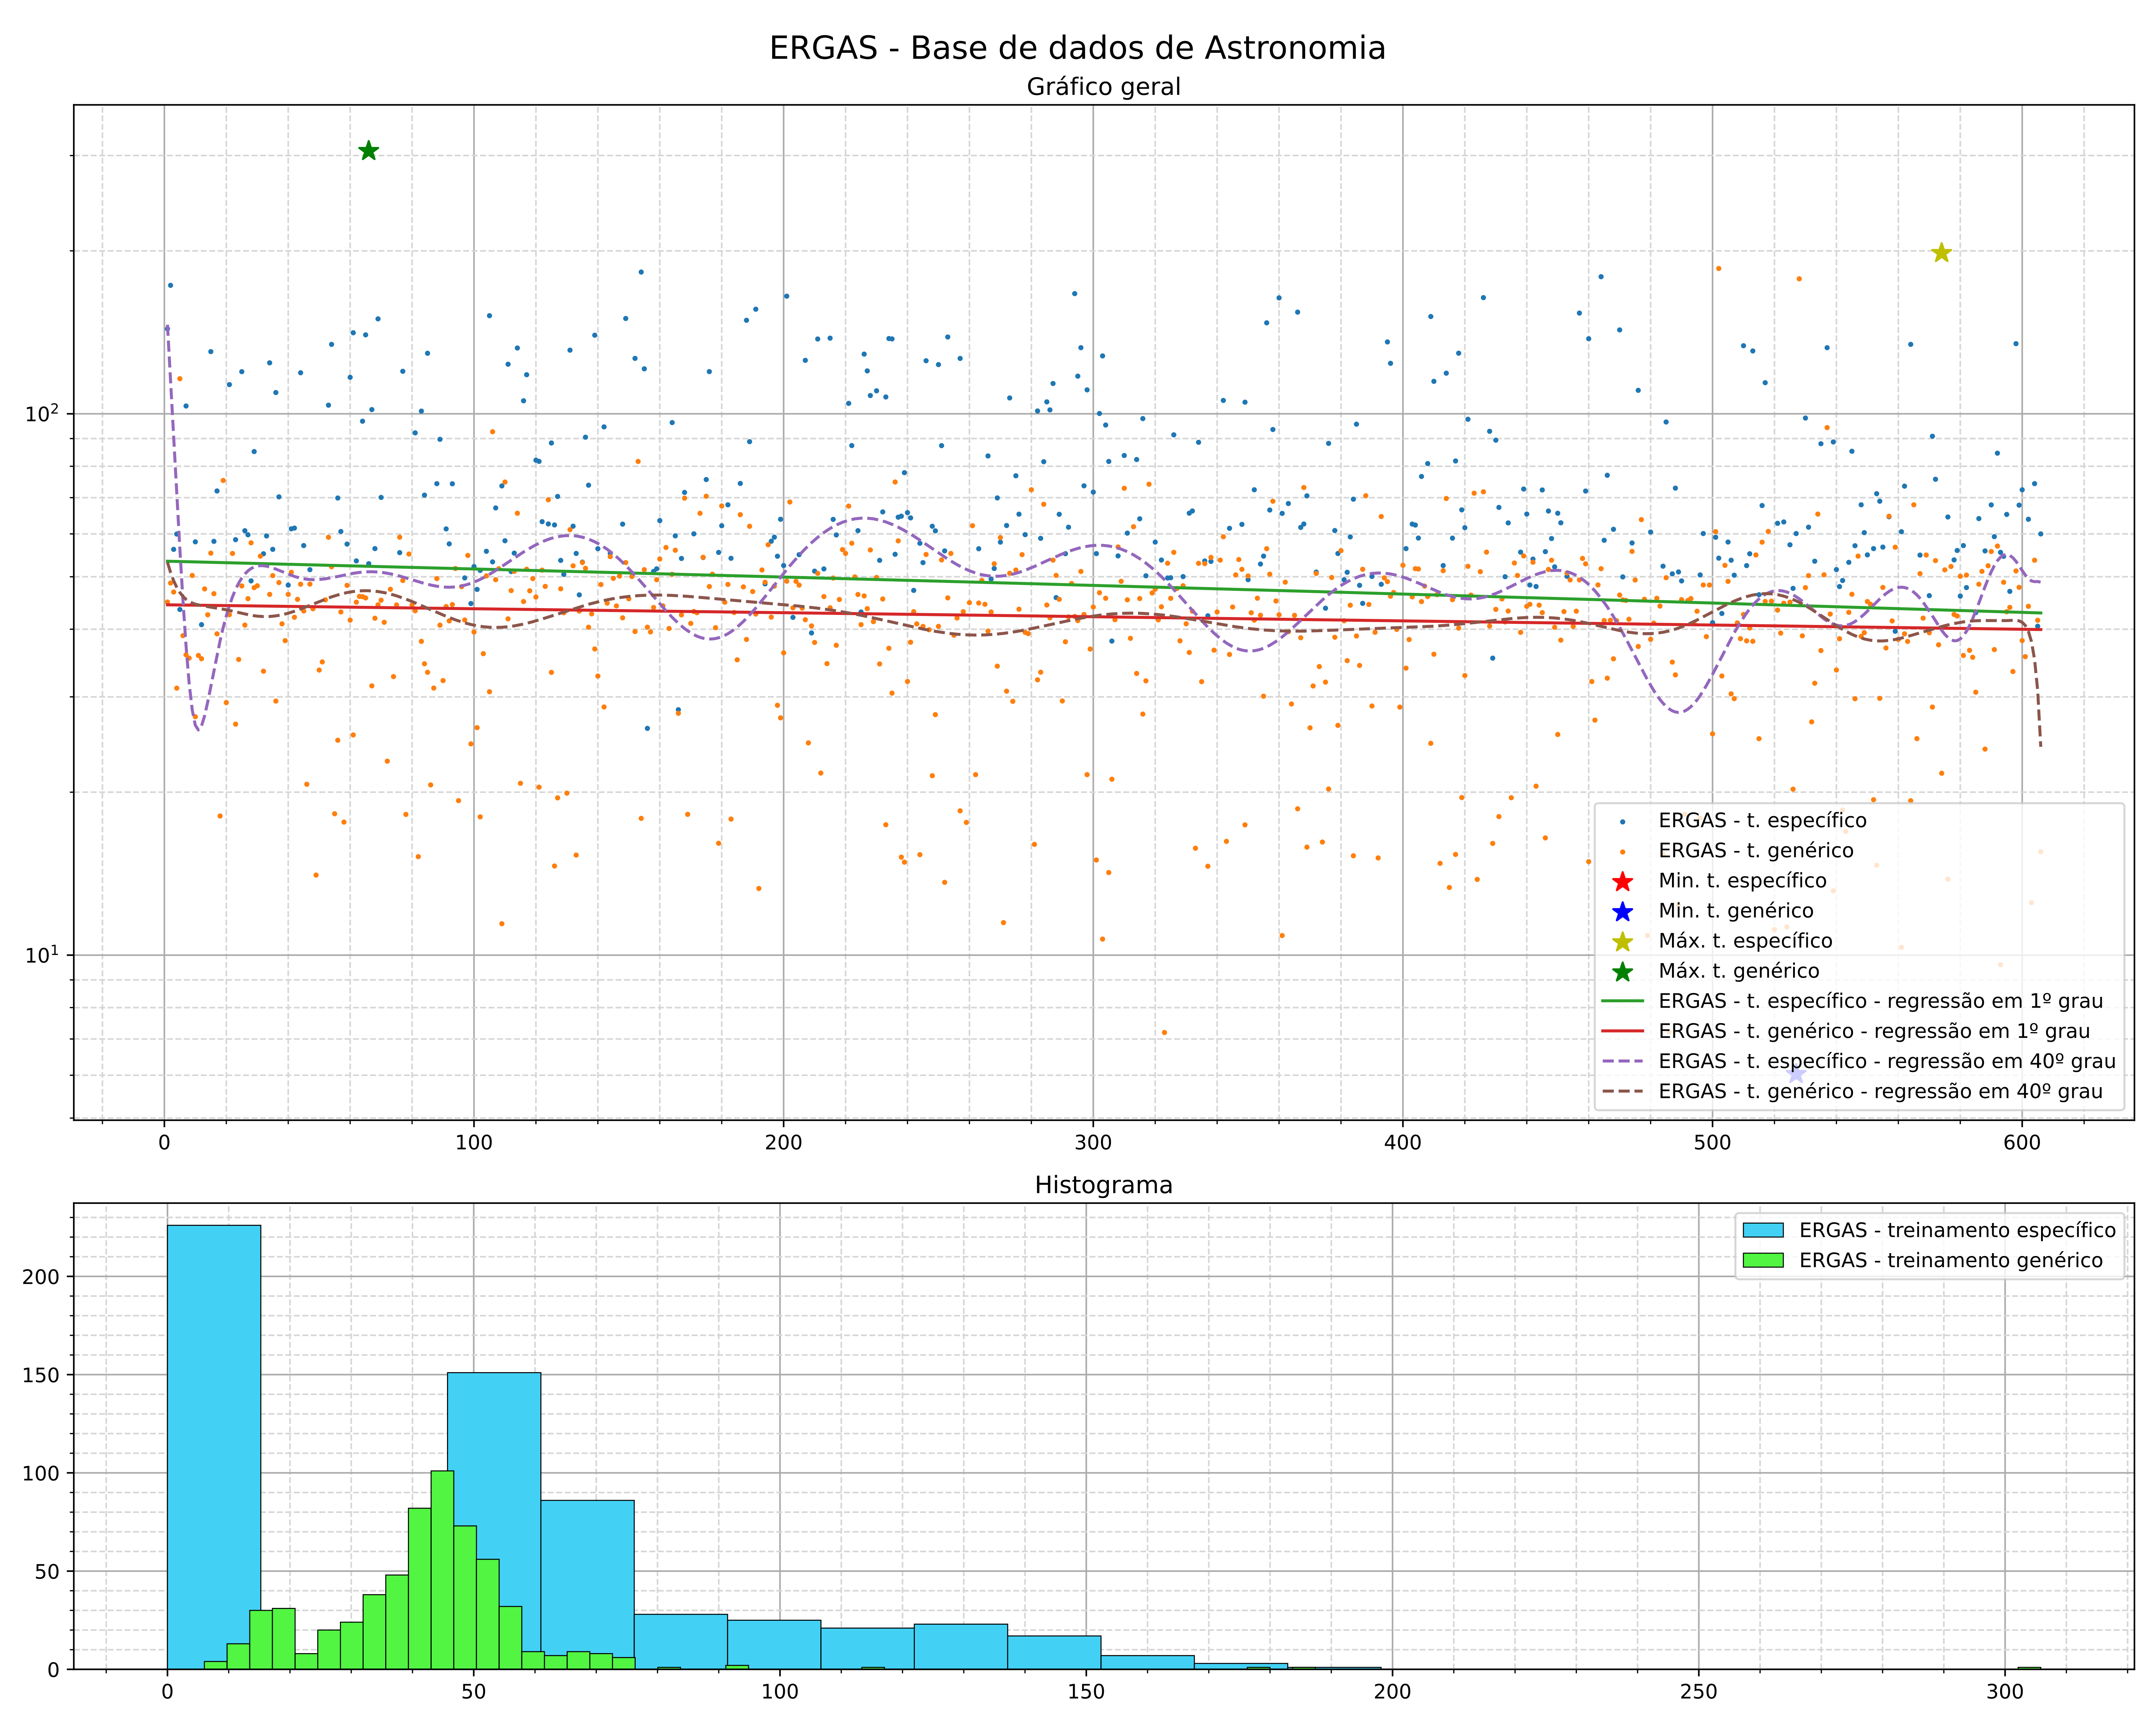
\includegraphics[width=10cm]{fig/resultados/astronomy/png/ergas_astronomy_compound.png}
    \legend{Fonte: Autor}
    \label{fig:results:fig8}
\end{figure}

Outra vez, na figura \ref{fig:results:fig8} o ETE é maior que o ETG e assim como no erro ERGAS da seção \ref{sec:result:mri:ergas}, a dispersão dificultaria a análise sem as regressões. Apesar disso, o resultado se mantém. O treinamento específico produziu imagens menos similares às originais.

\section{Considerações gerais sobre o resultado}
\label{sec:result:consideracoes-gerais}

No geral, o TE produziu resultados inferiores ao TG e isso foi fortemente evidenciado em cada um dos gráficos descritos anteriormente. Constante e consistentemente o ETG produziu erros menores que o ETE, excluindo naturalmente o PSNR em que a análise se inverte, e em consequência, o maior valor é o mais atraente, do ponto de vista de similaridade. Com os ajustes necessários, o ETE sempre apontou na direção de menor similaridade com as imagens originais e isso é notável até mesmo de forma subjetiva e visual, como demonstrado nas imagens \ref{fig:img-results:fig1} e \ref{fig:img-results:fig2} na seção \ref{sec:amostra-img-resultante}.
